\chapter{Control Estructural}


\section{Open-loop vs closed-loop control}
\subsection{Open-loop (feedforward)}
\begin{figure}[H]
\centering
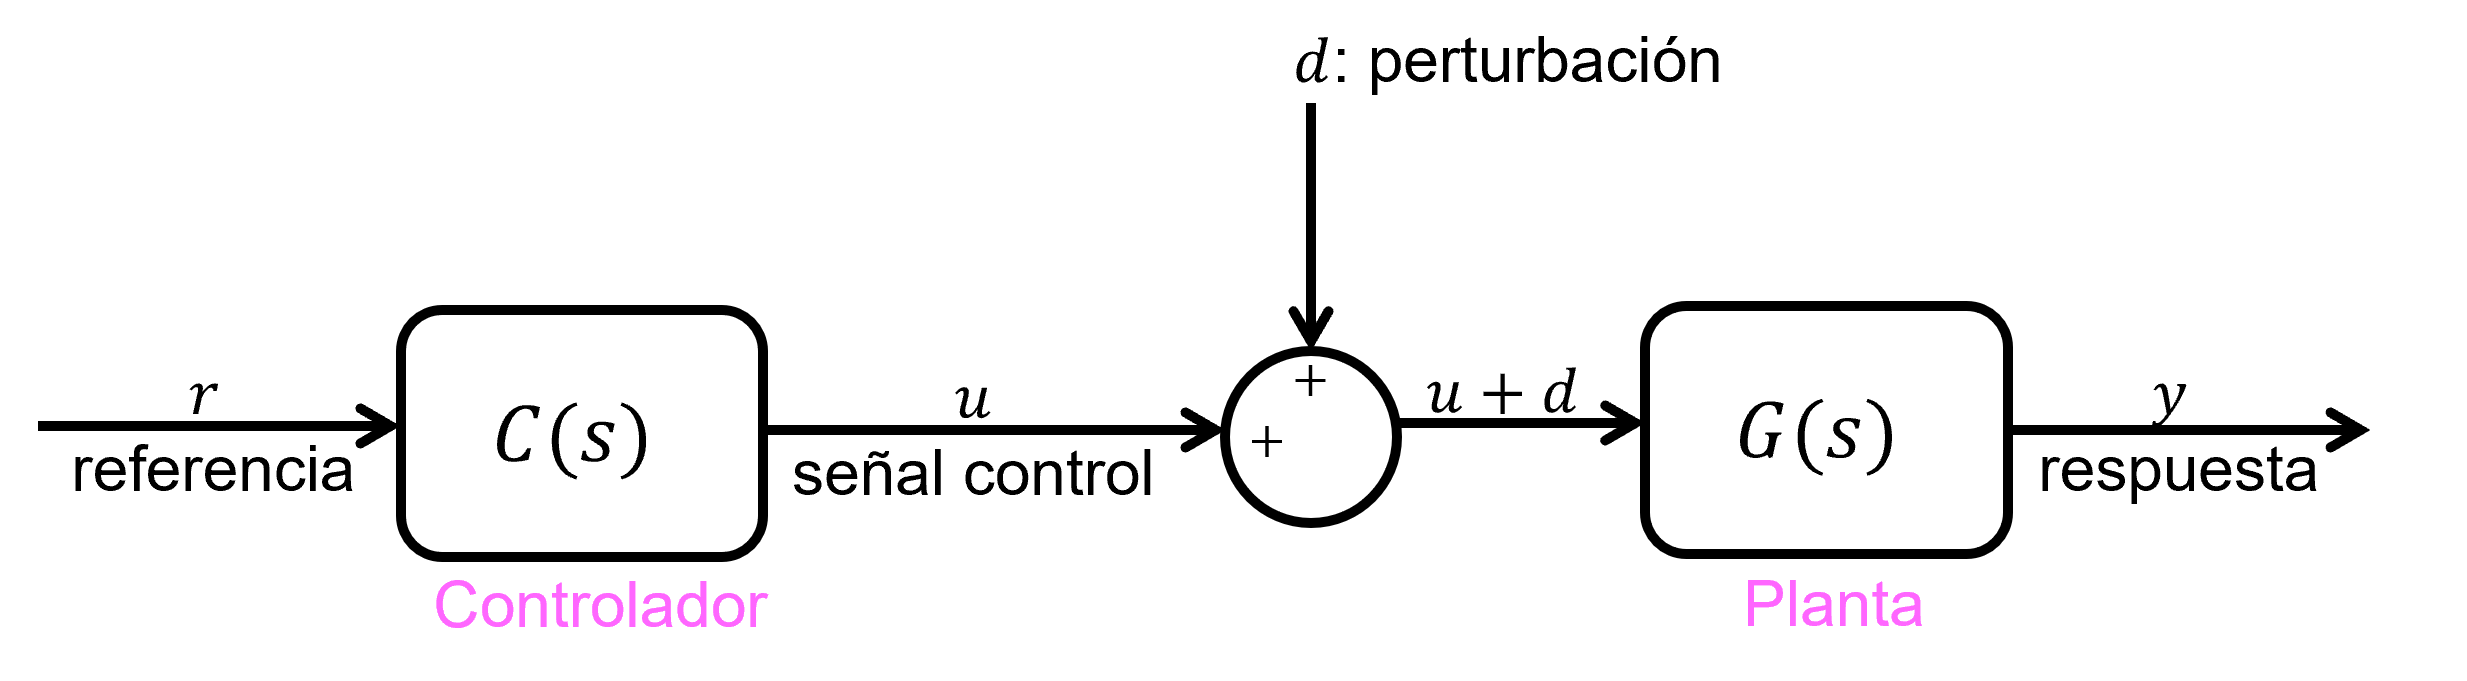
\includegraphics[scale=0.7]{Figuras/open-loop.png}
\end{figure}

\begin{itemize}
    \item[(1)] $Y(s)=G(s)[U(s)+D(s)]$, si asumimos $D(s)=0$
    \item[(2)] $U(s)=C(s)R(s)$
\end{itemize}

Reemplazar (2) en (1):
$$Y(s)=G(s)C(s)R(s)=L(s)R(s)$$
Donde $L(s)=G(s)C(s)$ es el sistema abierto ``open-loop system''.\\
\par Si buscamos: 
\begin{align*}
    y(t)&=r(t) ~/\color{red}{\mathcal{L}\{\cdot\}}\\
    Y(s)&=R(s)\\
    \Longrightarrow L(s)&=1\\
    \Longrightarrow C(s)&=\frac{1}{G(s)} ~\text{``control inverso''}
\end{align*}

\underline{Nota}: 
\begin{itemize}
    \item Muy simple y ``barato'' (no hay necesidad de sensores)
    \item No es robusto $\Longrightarrow$ si hay incertidumbre en $G(s)$
    \begin{align*}
        L(s)&=G(s)C(s)\neq 1\\
        &=[\hat{G}(s)+\Delta(s)]\frac{1}{\hat{G}(s)}\\
        &=1+\frac{\Delta(s)}{\hat{G}(s)}
    \end{align*}
\end{itemize}
\underline{Nota}: podría ser útil en RTHS, porque la respuesta es instantánea.

\subsection{Closed-loop (feedback) control}
\begin{figure}[H]
\centering
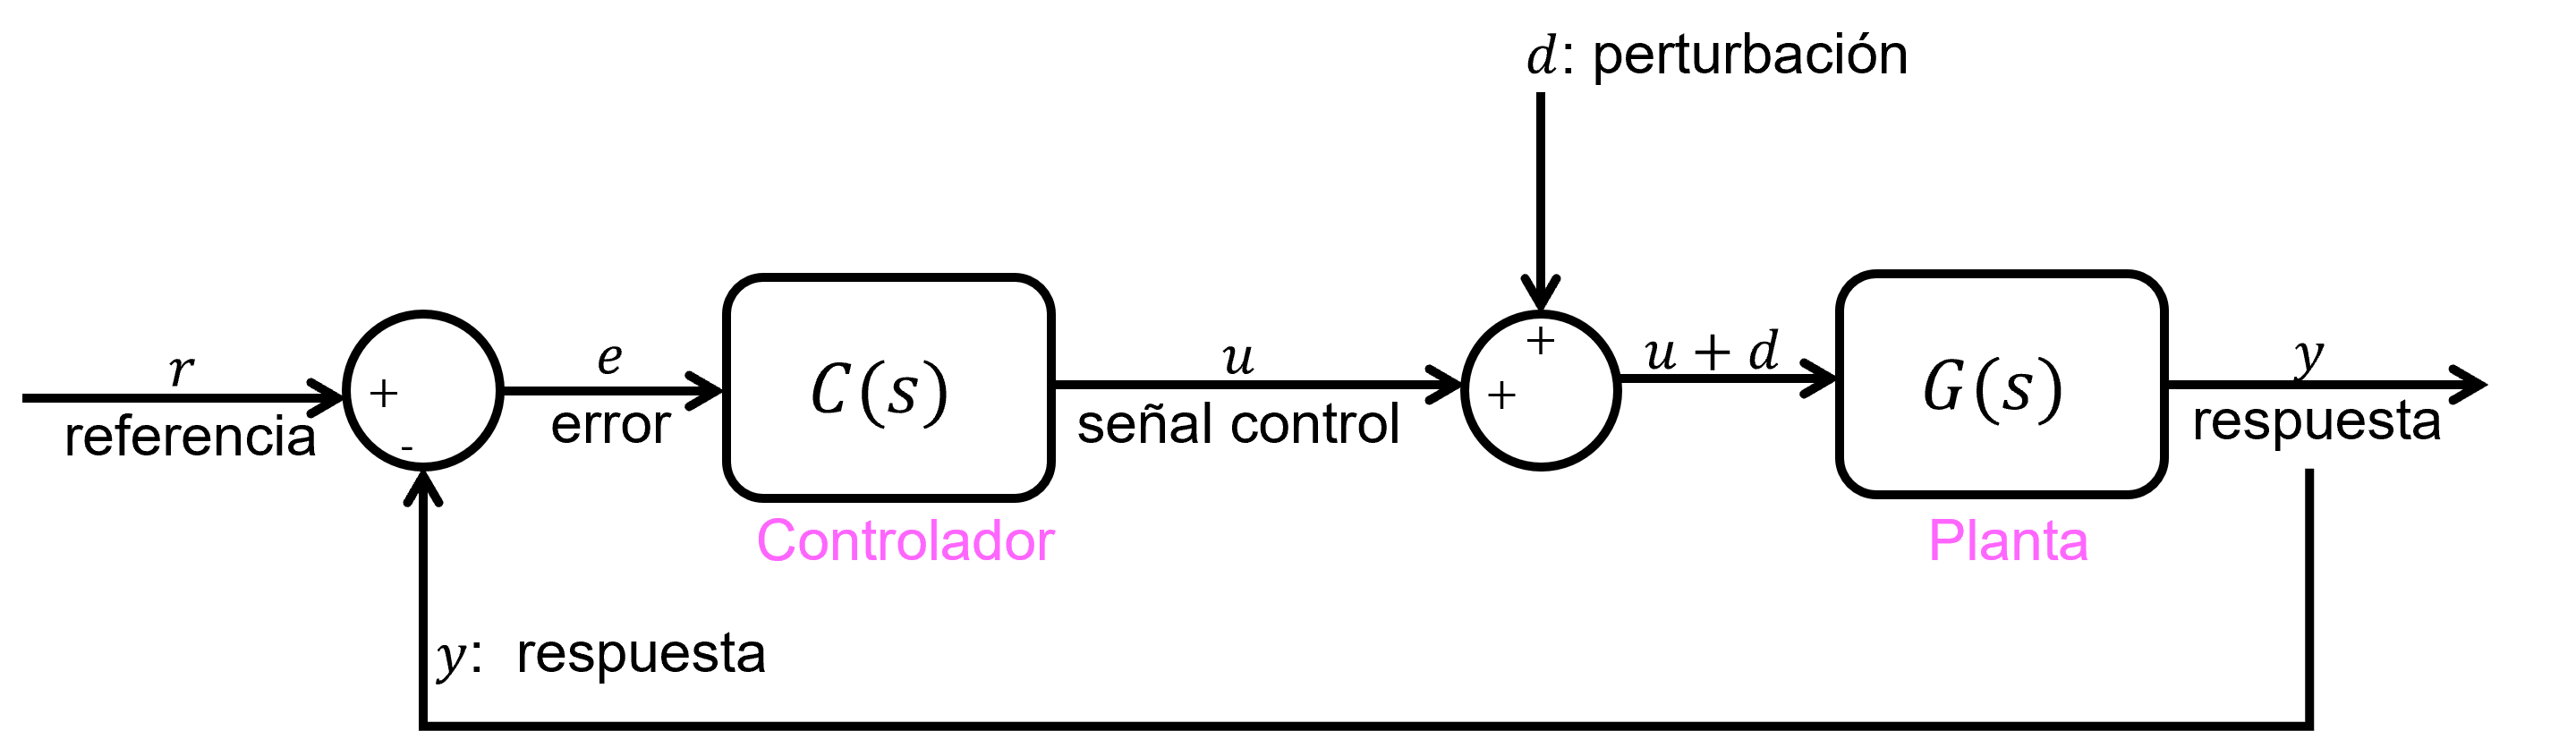
\includegraphics[scale=0.7]{Figuras/closed-loop.png}
\end{figure}

\begin{align*}
    \Longrightarrow & \text{Error: }~e(t)=r(t)-y(t)\\
    & \text{Si }e(t)=0\longrightarrow y(t)=r(t)
\end{align*}

\underline{Nota}:
\begin{itemize}
    \item Más robusto que feedforward $\Longrightarrow$ instalar sensores y ``alimentar'' la información de respuesta al controlador
    \item Más complicada y cara que open-loop
    \item Puede causar sistema estable o inestable
    \item Respuesta va a ser lenta $\Longrightarrow$ Real-time hybrid simulation
\end{itemize}

\section{Requisitos de control}
\begin{figure}[H]
\centering
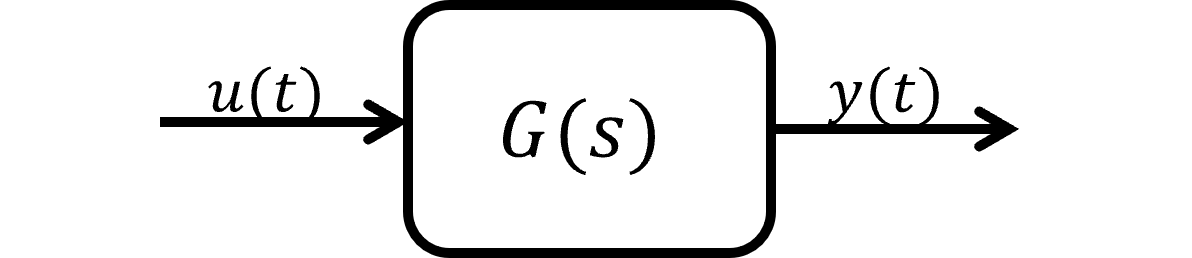
\includegraphics[scale=0.7]{Figuras/Planta.png}
\end{figure}
$\Longrightarrow$ Generar un set de requisitos de respuesta de planta $\Longrightarrow$ Especificaciones de respuesta transiente ante un escalón unitario
\begin{itemize}
    \item $t_r$ (tiempo de subida)
    \item $M_p$ (sobreimpulso)
    \item $t_s$ (tiempo de asentamiento)
\end{itemize}

\section{Diagrama de Bloque}
\begin{figure}[H]
\centering
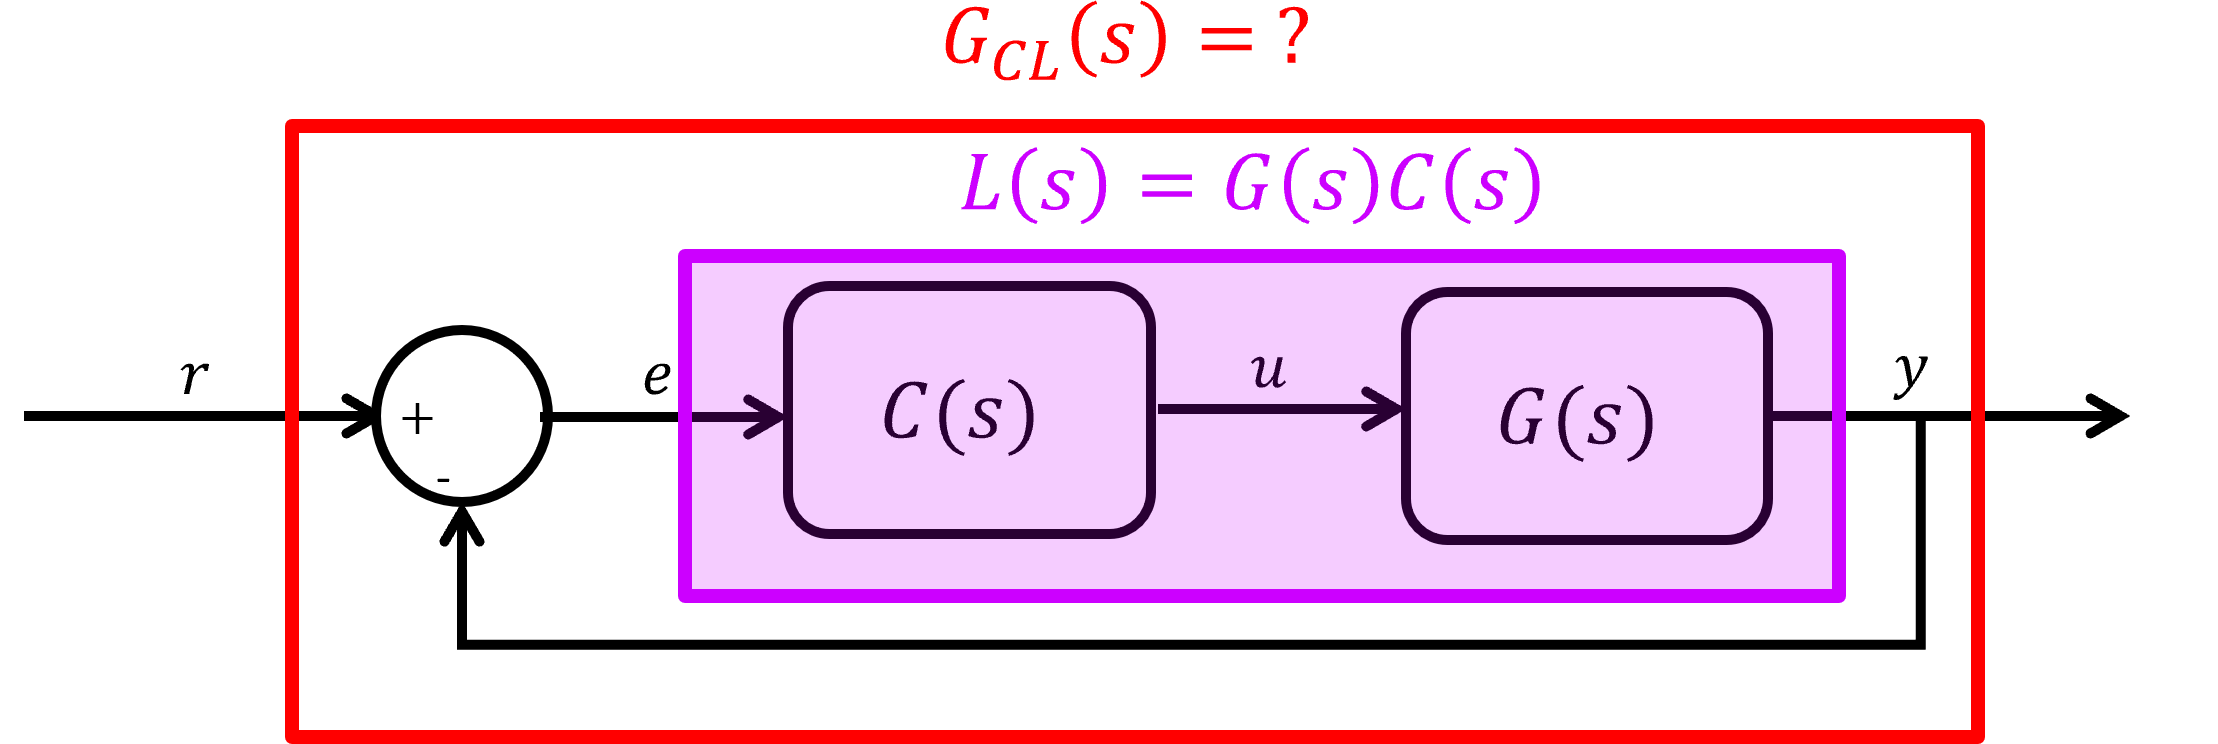
\includegraphics[scale=0.7]{Figuras/Diagrama_bloque.png}
\end{figure}
\begin{itemize}
    \item[(1)] $Y(s)=L(s)E(s)=G(s)C(s)E(s)$
    \item[(2)] $E(s)=R(s)-Y(s)$
\end{itemize}

(2) en (1): 
\begin{align*}
    \Longrightarrow Y(s)&=G(s)C(s)[R(s)-Y(s)]\\
    \Longrightarrow[1+G(s)C(s)]Y(s)&=G(s)C(s)R(s)\\
    \Longrightarrow Y(s)&= \bigg[\frac{G(s)C(s)}{1+G(s)C(s)}\bigg]R(s)\\
    \Longrightarrow Y(s)&= G_{CL}(s)R(s)
\end{align*}

\underline{Nota}: Vamos a ajustar $C(s)$ tal que $G_{CL}(s)$ tenga las propiedades deseadas en función de $t_r$, $M_p$ y $t_s$. O bien, elegir posición de los polos de $G_{CL}(s)$.





\section{Teorema Límite Final}
\begin{figure}[H]
\centering
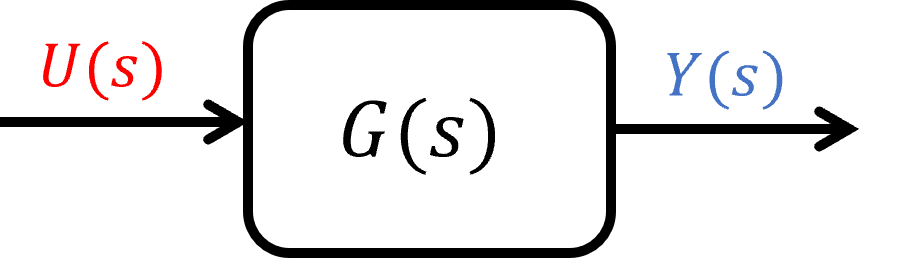
\includegraphics[scale=0.7]{Figuras/planta2.png}
\end{figure}
Respuesta Estado Estacionario: $y_\infty=\lim_{t\to\infty} y(t)$\\
\par Válido si y solo si $G(s)$ es estable.\\
\par \underline{Teorema}: Si todos los polos de $G(s)$ se encuentran a la izquierda del plano complejo, entonces:
\begin{align*}
    \lim_{t\to\infty} y(t)=\lim_{s\to 0} sY(s)
\end{align*}
\section{Sistema estructural con Active Mass Damper (AMD)}
\begin{figure}[H]
\centering
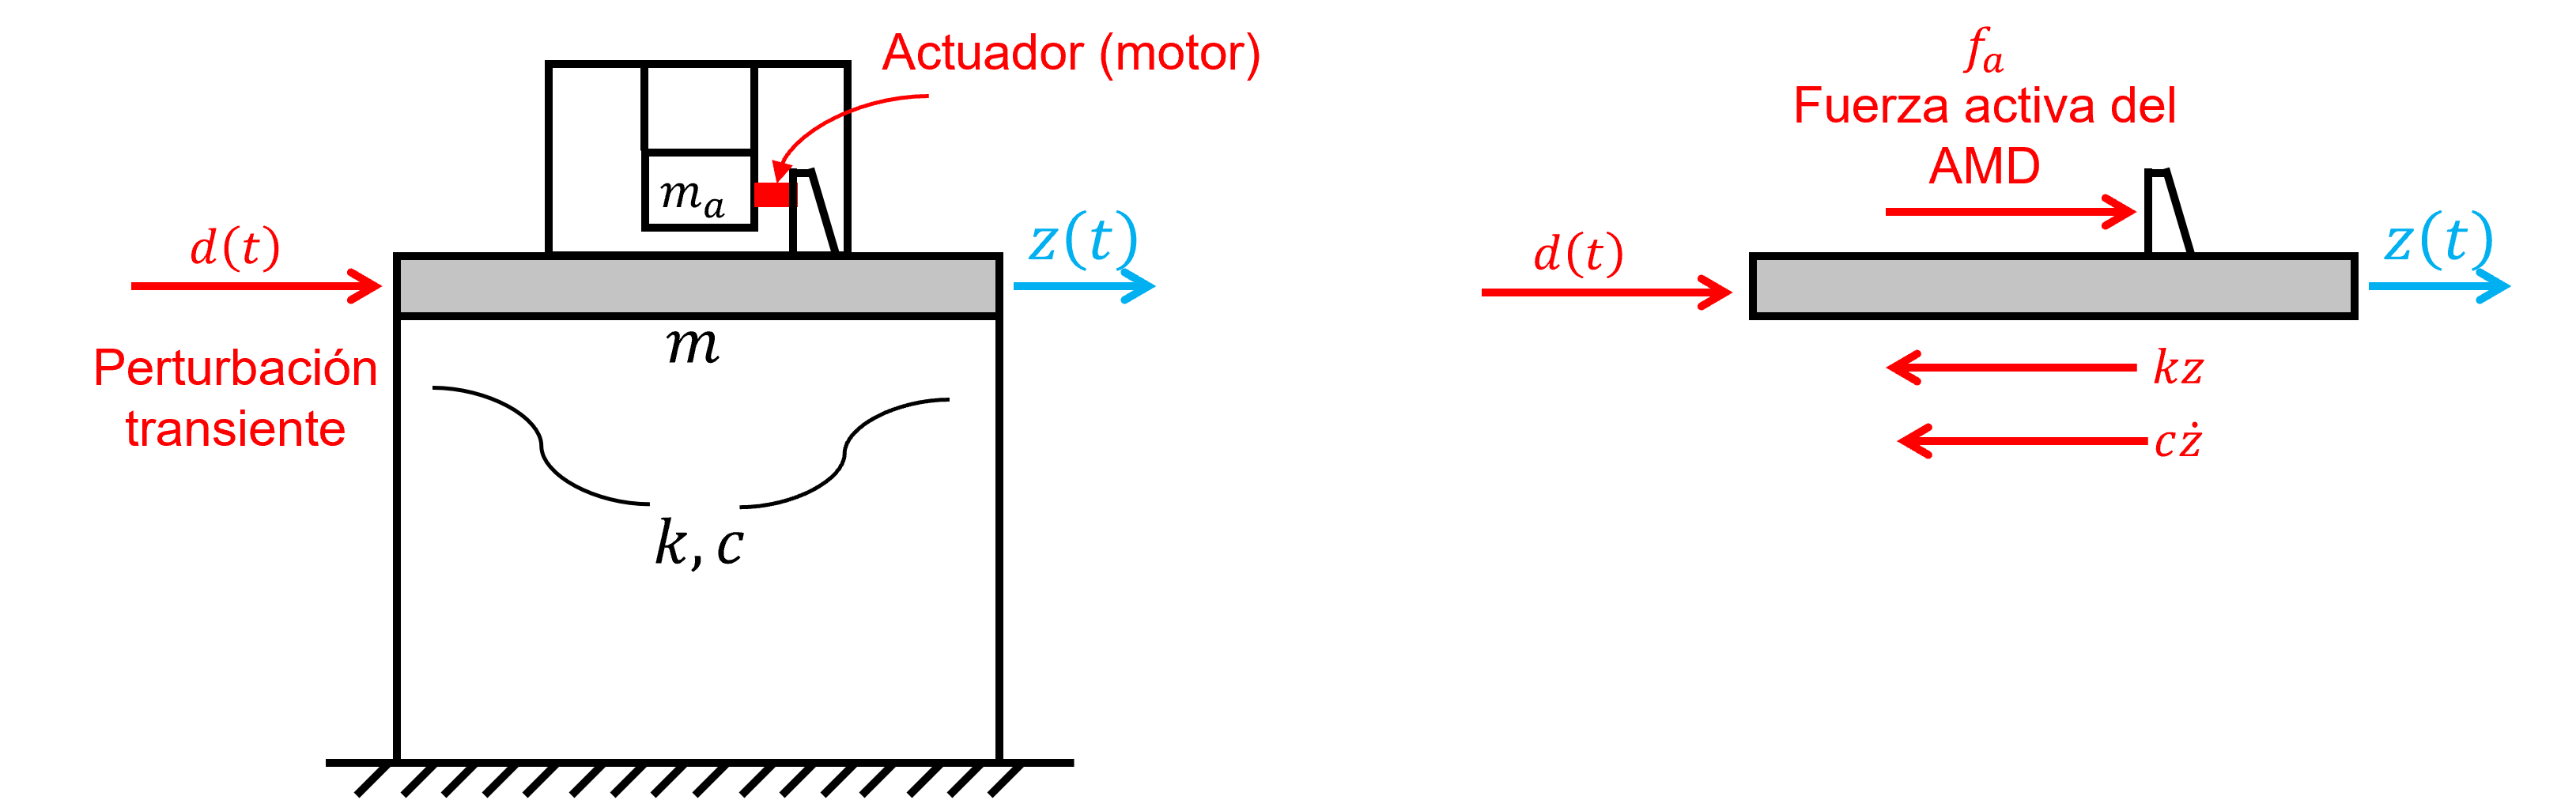
\includegraphics[scale=0.7]{Figuras/AMD.png}
\end{figure}
\begin{align*}
    \text{EDM: }~ m\ddot{z}+c\dot{z}+kz=f_a(u)+\cancelto{\text{Asuma=0}}{d}
\end{align*}
$u$: señal control (voltaje)\\
\par \underline{Objetivo}: Diseñar un \textcolor{red}{sistema de control} para mitigar $z(t)$ $\Longrightarrow$ Control PID (Proporcional-Integral-Derivativo)

\section{Control PID}
\begin{align*}
    C(s)=K_p+K_Ds+\frac{K_I}{s}
\end{align*}
\begin{itemize}
    \item $K_p$: control proporcional
    \item $K_D$: control derivativo
    \item $K_I$: control integral
\end{itemize}

\begin{figure}[H]
\centering
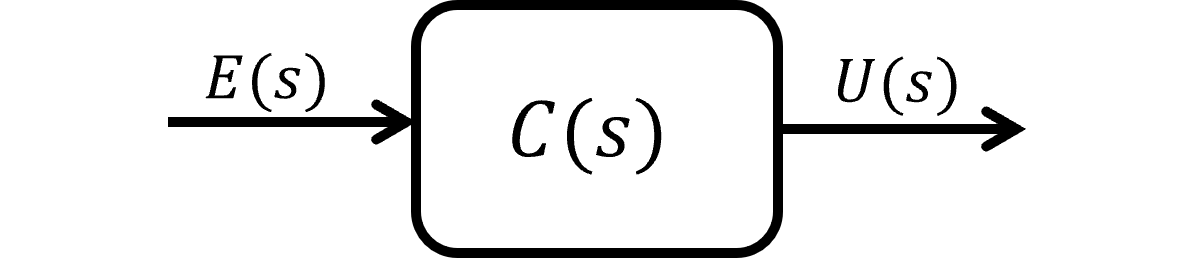
\includegraphics[scale=0.7]{Figuras/controlador.png}
\end{figure}

\begin{align*}
    U(s)&=C(s)E(s)\\
    &=K_pE(s)+K_DsE(s)+K_I\frac{E(s)}{s}~/\color{red}{\mathcal{L}^{-1}\{\cdot\}}\\
    \Longrightarrow u(t)&=K_pe(t)+K_D\frac{de(t)}{dt}+K_I\int e(t)dt
\end{align*}
 
\begin{itemize}
    \item $K_pe(t)$: error instantáneo
    \item $K_D\frac{de(t)}{dt}$: error futuro
    \item $K_I\int e(t)dt$: error pasado
\end{itemize}

\begin{figure}[H]
\centering
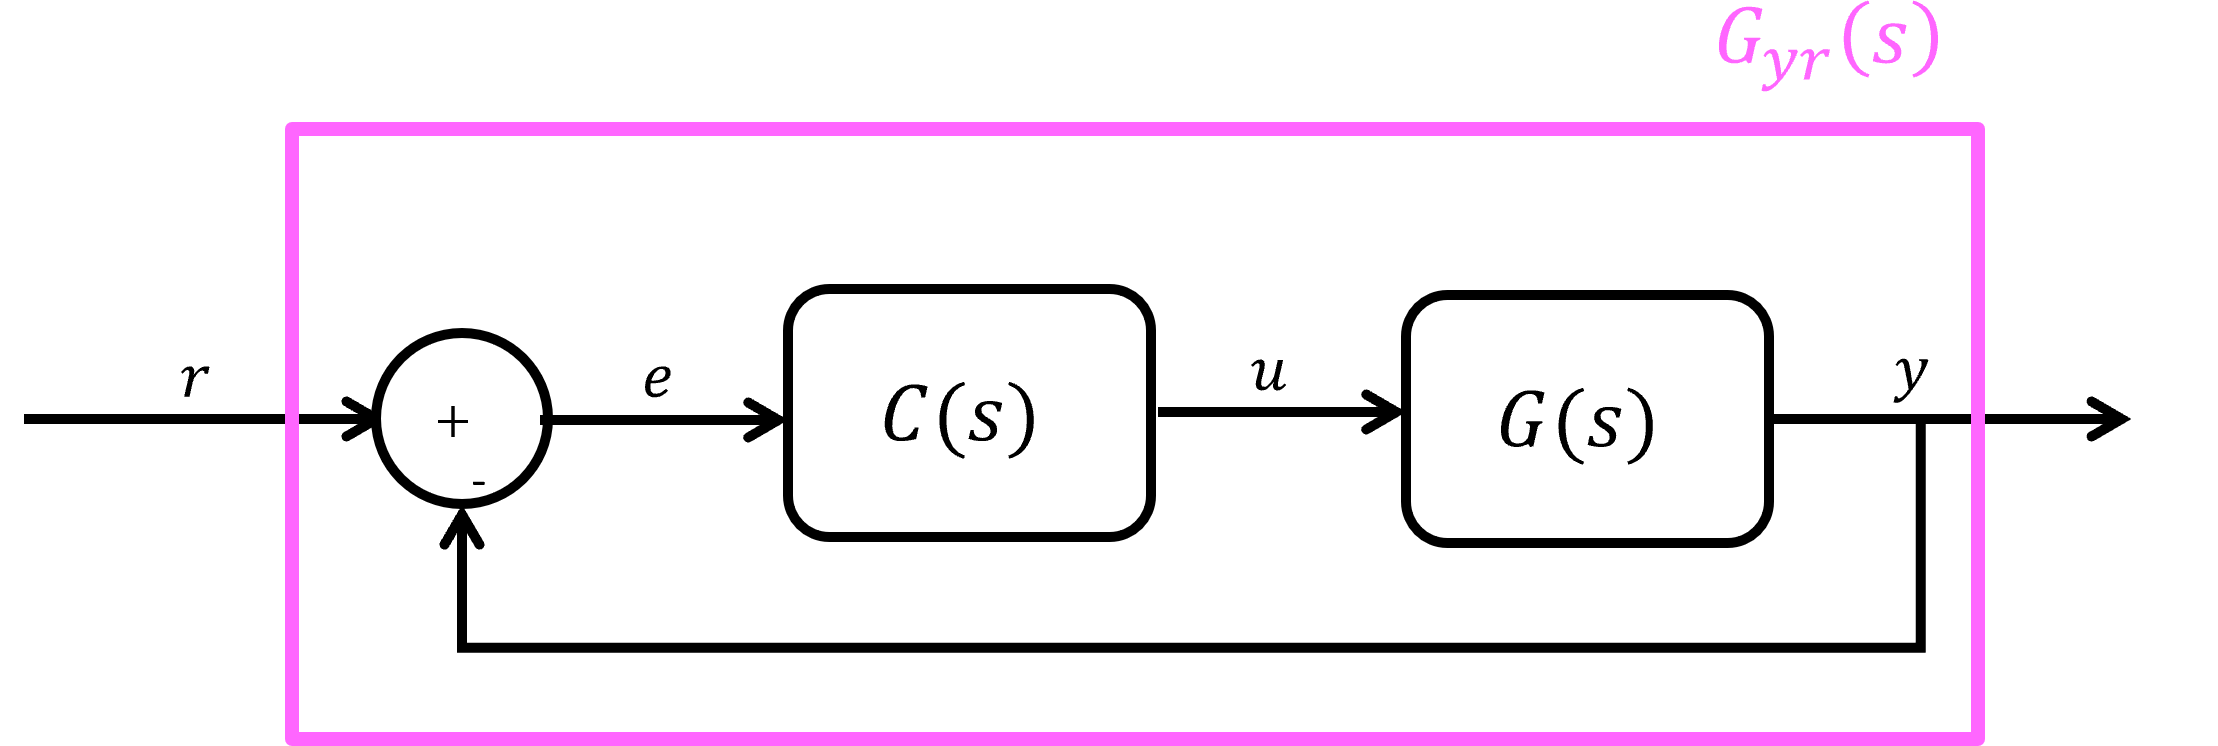
\includegraphics[scale=0.7]{Figuras/PID2.png}
\end{figure}
$C(s)$ se diseña tal que $e(t)\to 0$
$$C(s)=K_p+\frac{K_I}{s}+K_Ds$$
\begin{itemize}
    \item $Y(s)=G(s)U(s)$
    \item $U(s)=C(s)E(S)$
    \item $E(s)=R(s)-Y(s)$
\end{itemize}
\begin{align*}
    Y(s)&=G(s)C(s)[R(s)-Y(s)]\\
    \Longrightarrow Y(s)&=\frac{G(s)C(s)}{1+G(s)C(s)}R(s)\\
    &=G_{CL}R(s)\\
    &=G_{yr}R(s)
\end{align*}

\subsection{Control Proporcional (P)}
\begin{align*}
    & C(s)=K_p\\
    \Longrightarrow & G(s)=\frac{1}{ms^2+cs+k}=\frac{1/m}{s^2+2\xi\omega_n s+\omega_n^2}=\frac{c}{s^2+as+b}\\
    \Longrightarrow & G_{CL}(s)=\frac{K_p\frac{c}{s^2+bs+c}}{1+K_p\frac{c}{s^2+bs+c}}
\end{align*}
\begin{align*}
    \Longrightarrow & G_{CL}(s)=\frac{K_p c}{s^2+as+(b+K_p\cdot c)}\\
    \Longrightarrow & \omega_{n,CL}= \sqrt{b+K_p\cdot c}\\
    \Longrightarrow & \xi_{CL}= \frac{a}{2\omega_{n,CL}}=\frac{a}{2\sqrt{b+K_p\cdot c}}
\end{align*}
\begin{itemize}
    \item Aumentar $K_p$ hace que $\omega_{n,CL}$ aumente (sistema rígido)
    \item Aumentar $K_p$ hace que $\xi$ disminuya
\end{itemize}

En términos de la respuesta $y_{\infty}$: 
\begin{align*}
    y_{\infty}=\lim_{s\to 0}sY_{CL}(s)=\lim_{s\to 0} sG_{CL}(s)R(s)
\end{align*}
Con $R(s)$: escalón unitario

\begin{align*}
    \Longrightarrow y_{\infty}=\lim_{s\to 0} s\frac{K_p\cdot c}{s^2+as+(b+K_p\cdot c)}\cdot\frac{1}{s}=\frac{K_p\cdot c}{b+K_p \cdot c}\neq 1
\end{align*}
Valores pequeños de $K_p\Longrightarrow$ error en estado estacionario
\begin{figure}[H]
\centering
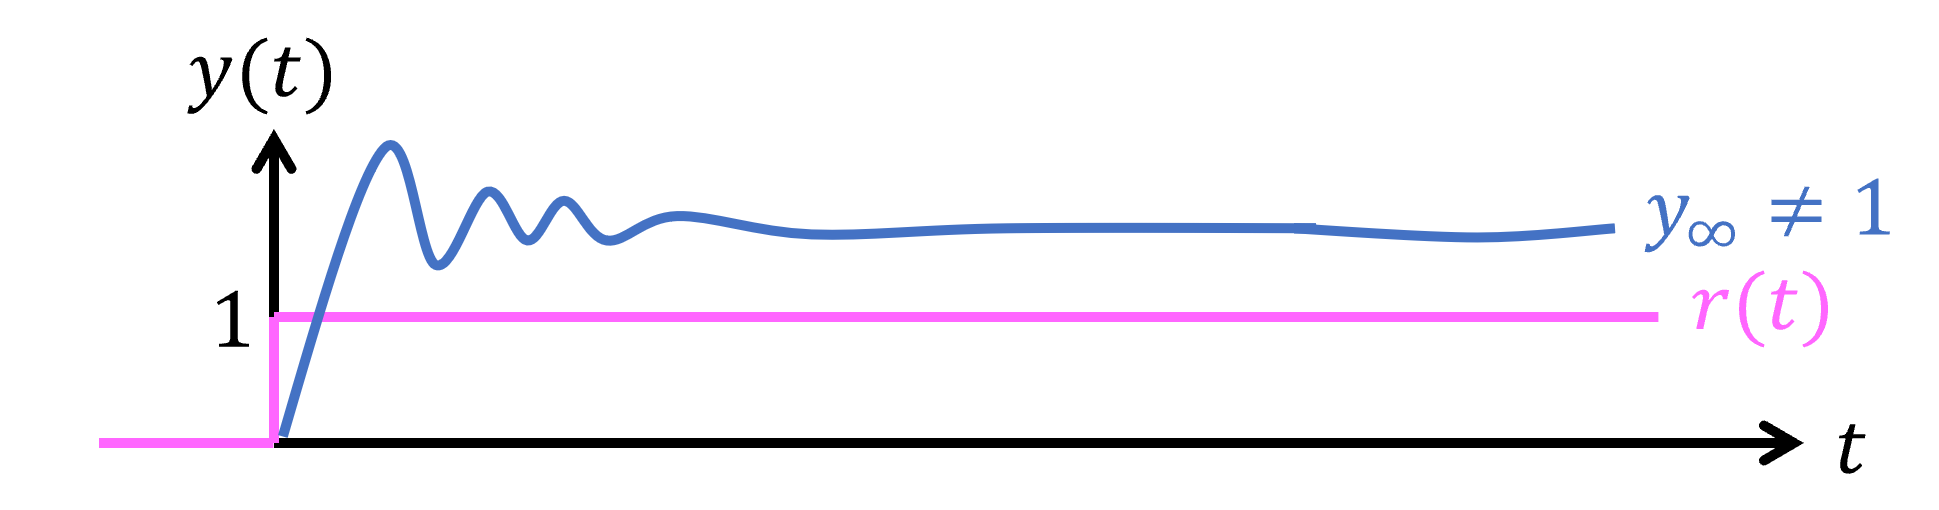
\includegraphics[scale=0.7]{Figuras/controlP.png}
\end{figure}

\subsection{Control PD}
\begin{align*}
    G_{CL}(s)&=\frac{G(s)C(s)}{1+G(s)C(s)}=\frac{\left(\frac{c}{s^2+as+b}\right)C(s)}{1+\left(\frac{c}{s^2+as+b}\right)C(s)}\\
    & = \frac{c\cdot C(s)}{a^2+as+\left( b+c \cdot C(s) \right)}\\
    C(s) &= K_p+K_Ds=K_p(1+T_Ds)\\
    \Longrightarrow G_{CL} &= \frac{cK_p(1+T_Ds)}{s^2+(a+cbK_pT_D)s+b(1+K_p)}
\end{align*}

\begin{itemize}
    \item Aparece un ``cero'' en el numerador
    \item Podemos controlar $\omega_{n,CL}$ mediante $K_p$
    \item Podemos controlar $\xi_{CL}$ mediante una combinación de $K_p$ y $T_D$
\end{itemize}

$\Longrightarrow y_{\infty}$, no hay cambio en el error de estado estacionario\\
\par $\Longrightarrow$ Con PD podemos ubicar los polos del sistema cerrado donde nosotros queramos\\
\par \underline{Advertencia}: Control D amplifica el ruido eléctrico en la señal de respuesta $\Longrightarrow$ Nunca utilizar control D.

\subsection{Control PI}
\begin{align*}
    \Longrightarrow G_{CL}(s) &= \frac{c\cdot C(s)}{s^2+as+\left(b+c \cdot C(s)\right)}\\
    \Longrightarrow C(s) &= K_p +\frac{K_I}{s}=K_P\left(1+\frac{T_I}{2}\right)\\
    \Longrightarrow G_{CL} &= \frac{cK_p(s+T_I)}{s^3+as^2+(b+cK_p)s+cK_pT_I}
\end{align*}

\begin{align*}
    \Longrightarrow y_{\infty}=\lim_{s\to 0}sY_{CL}(s)=\lim_{s\to 0} s\frac{K_p\cdot c(s+T_I)}{s^3+as^2+(b+cK_p)s+cK_pT_I}\cdot\frac{1}{s}=\frac{T_IK_p\cdot c}{T_IK_p\cdot c}= 1
\end{align*}

\underline{Nota}: El esfuerzo del control I genera una reducción del error en estado estacionario.

\subsection{Control PID}
\begin{align*}
    C(s) &= K_p+\frac{K_I}{s}+K_Ds\\
    &= K_p\left(1+\frac{T_I}{s}+T_Ds\right)
\end{align*}

\begin{itemize}
    \item Aumentar $K_p$: Sistema que responde rápido, pero se genera alto sobreimpulso, y el error estacionario alto.
    \item Aumentar $K_D$: Agregar amortiguameinto al sistema (disminuir sobreimpulso), pero puede amplificar el ruido eléctrico.
    \item Aumentar $K_I$: Reducir el error en estado estacionario, sistema se vuelve más lento.
\end{itemize}

\begin{table}[H]
    \centering
    \begin{tabular}{c|c|c|c|}
                & $K_p \uparrow$ & $K_D \uparrow$ & $K_I \uparrow$\\ \hline
         error ss & $\downarrow$ & - & 0\\ \hline
         $t_r$ & $\downarrow$ & - & ? \\ \hline
         $t_s$ & - & $\downarrow$ & ? ($\uparrow$)\\ \hline
         $M_p$ & $\uparrow$ & $\downarrow$ & ? ($\uparrow$)\\ 
    \end{tabular}
\end{table}



\section{Ejemplo: Simulación mediante Simulink}
\begin{figure}[H]
\centering
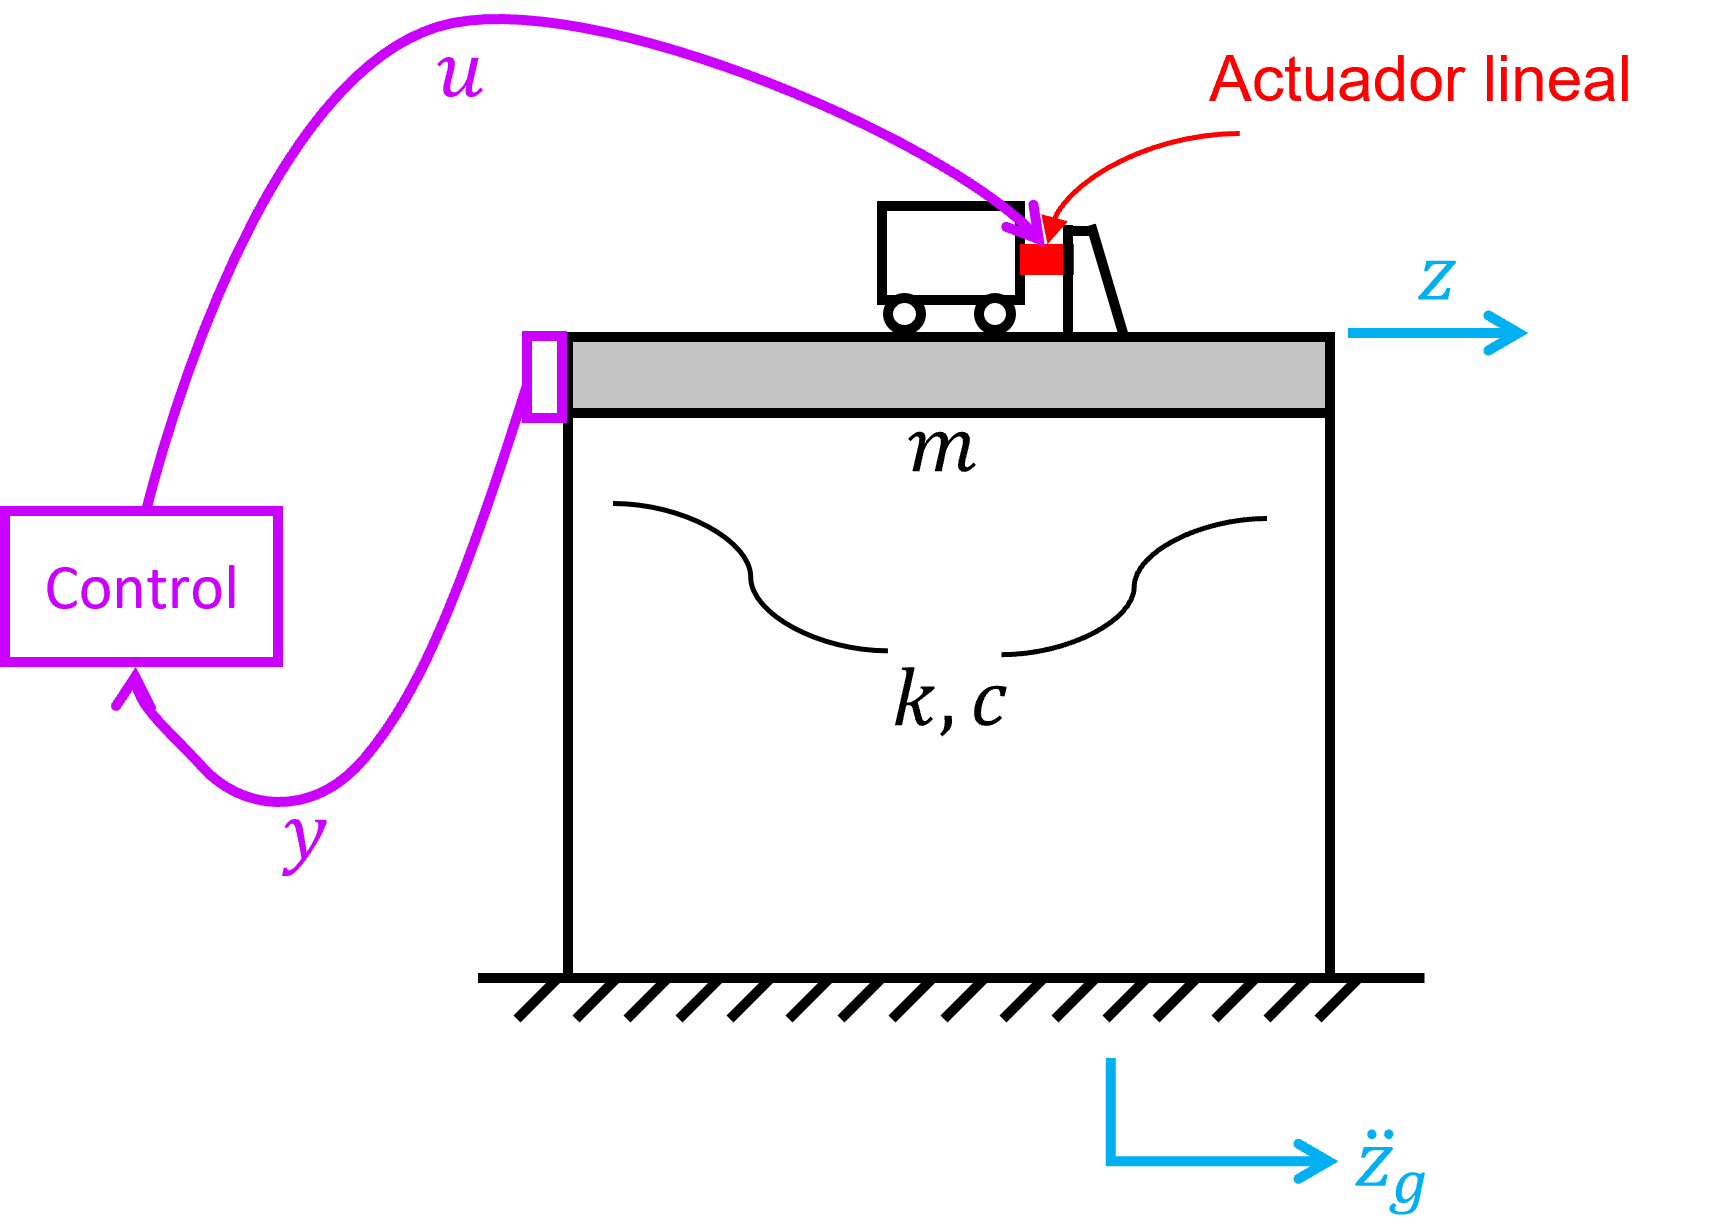
\includegraphics[scale=0.7]{Figuras/simulink_modelo.png}
\end{figure}

\begin{align*}
    \text{EDM: }~ m\ddot{z}+c\dot{z}+kz=-m\ddot{z}_g+gu
\end{align*}

\underline{Propiedades de la estructura}: 
\begin{itemize}
    \item $m=100$ Kg
    \item $c=50$ Ns/m
    \item $k=4000$ N/m
    \item $g=100$ N/V
\end{itemize}

\underline{Representación espacio-estado}: 
\begin{align*}
    \tend{x}=\begin{bmatrix}\tend{z}\\ \tend{\dot{z}}\end{bmatrix}, \quad u_1 =\ddot{z}_g, \quad u_2=u
\end{align*}

\begin{align*}
    \tend{\dot{x}} &=
    \begin{bmatrix}
    0 & 1\\
    -k/m & -c/m
    \end{bmatrix}\tend{x} +
    \begin{bmatrix}
    0 \\ -1
    \end{bmatrix}u_1+
    \begin{bmatrix}
    0 \\ g/m
    \end{bmatrix}u_2 \\
    &= \begin{bmatrix} 0 & 1\\-k/m & -c/m
    \end{bmatrix}\tend{x} +
    \begin{bmatrix}
    0 & 0\\ -1 & g/m
    \end{bmatrix} 
    \begin{bmatrix}
    \ddot{z}_g\\ u
    \end{bmatrix}
\end{align*}

\begin{align*}
    \tend{y}&=[z]\\
    \tend{y}&= \begin{bmatrix}1 & 0 \end{bmatrix}\tend{x}+\begin{bmatrix}0 & 0 \end{bmatrix}\begin{bmatrix}
    \ddot{z}_g\\ u
    \end{bmatrix}
\end{align*}

\begin{align}
    \tend{u}=\begin{bmatrix}
    \ddot{z}_g\\ u
    \end{bmatrix}\longrightarrow
    \begin{array} {|r|r|}
      \hline A & B \\
      \hline C & D \\
      \hline 
    \end{array}
    \longrightarrow \tend{y}=[z] \quad \text{Sistema ``MISO''}
\end{align}


\underline{Objetivo}: Diseñar un control PID para mejorar el desempeño de la estructura sometida al terremoto de Northridge 1994.\\
\par \underline{Contol PID}: 
\begin{align*}
    C(s)&=K_p\bigg(1+\frac{T_I}{s}+T_Ds\bigg)\\
    &= K_p+\frac{K_I}{s}+K_Ds, \quad K_I=K_pT_I, \quad K_D=K_pT_D
\end{align*}

\begin{multicols}{2}
\underline{Código Matlab}: 
\begin{minted}[]{matlab}
%% Simulacion Control PID
% Gaston Fermandois, 2020

%% Inicializar
clear all, close all, clc

%% Parametros

m=100; % masa primer piso, kg
c=50; %Ns/m
k=4000; %N/m
g=100; %cte motor, N/V

%% Control PID

Kp=1;
Ti=1/10; Ki=Kp*Ti;
Td=1/100; Kd=Kp*Td;

s=tf('s');
Cpid=Kp*(1+Ti/s+Td*s);

%% Espacio estado

A=[0 1;-k/m -c/m];
B1=[0;-1];
B2=[0;g/m];
B=[B1 B2];
C=[1 0];
D1=0;
D2=0;
D=[D1 D2];

sys=ss(A,B,C,D);

sysyu=ss(A,B2,C,D2);

Gyu=tf(sysyu);

%% Sistema Cerrado

Gcl=Gyu*Cpid/(1+Gyu*Cpid);
Gcl=minreal(Gcl)

figure;
rlocus(Gcl)

%% Simulacion

Tfinal=60; %s
Fs=1000; %Hz
Ts=1/Fs; %s

GM=importdata('RegistroNorthridge1994.txt');
N=length(GM.data);
dt=0.02; %s
t=linspace(0,N*dt,N);
ddzg=[t.' GM.data/100]; %[s m/s2]

sim('AMDctrl_demo_simu')
\end{minted}
\end{multicols}
\underline{Simulink}:
\begin{figure}[H]
\centering
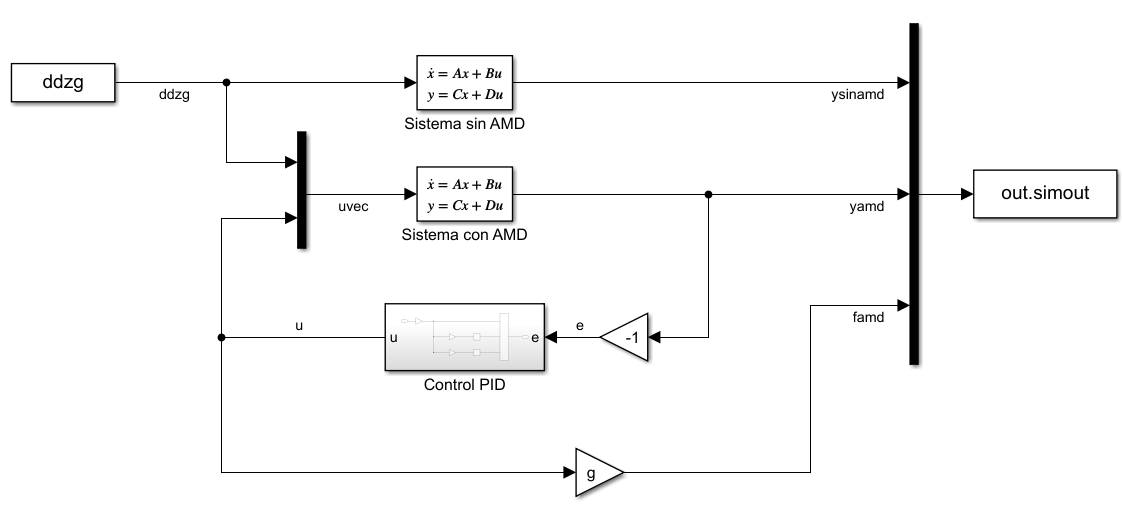
\includegraphics[scale=0.7]{Figuras/Simulink.png}
\end{figure}



\section{Root Locus}
$\Longrightarrow$ ``Migración de polos'', Locus = posición en latín
\begin{align*}
    \text{Planta: }~ G_{y\ddot{z}_g}(s)&=\frac{1/m}{s^2+2\xi\omega_n s+\omega_n^2}\\
    G_{yu}(s) &=\frac{g/m}{s^2+2\xi\omega_n s+\omega_n^2}
\end{align*}
\begin{align*}
    \text{Controlador PID: }~C(s)=K_p(1+\frac{T_I}{s}+T_Ds)
\end{align*}

\begin{figure}[H]
\centering
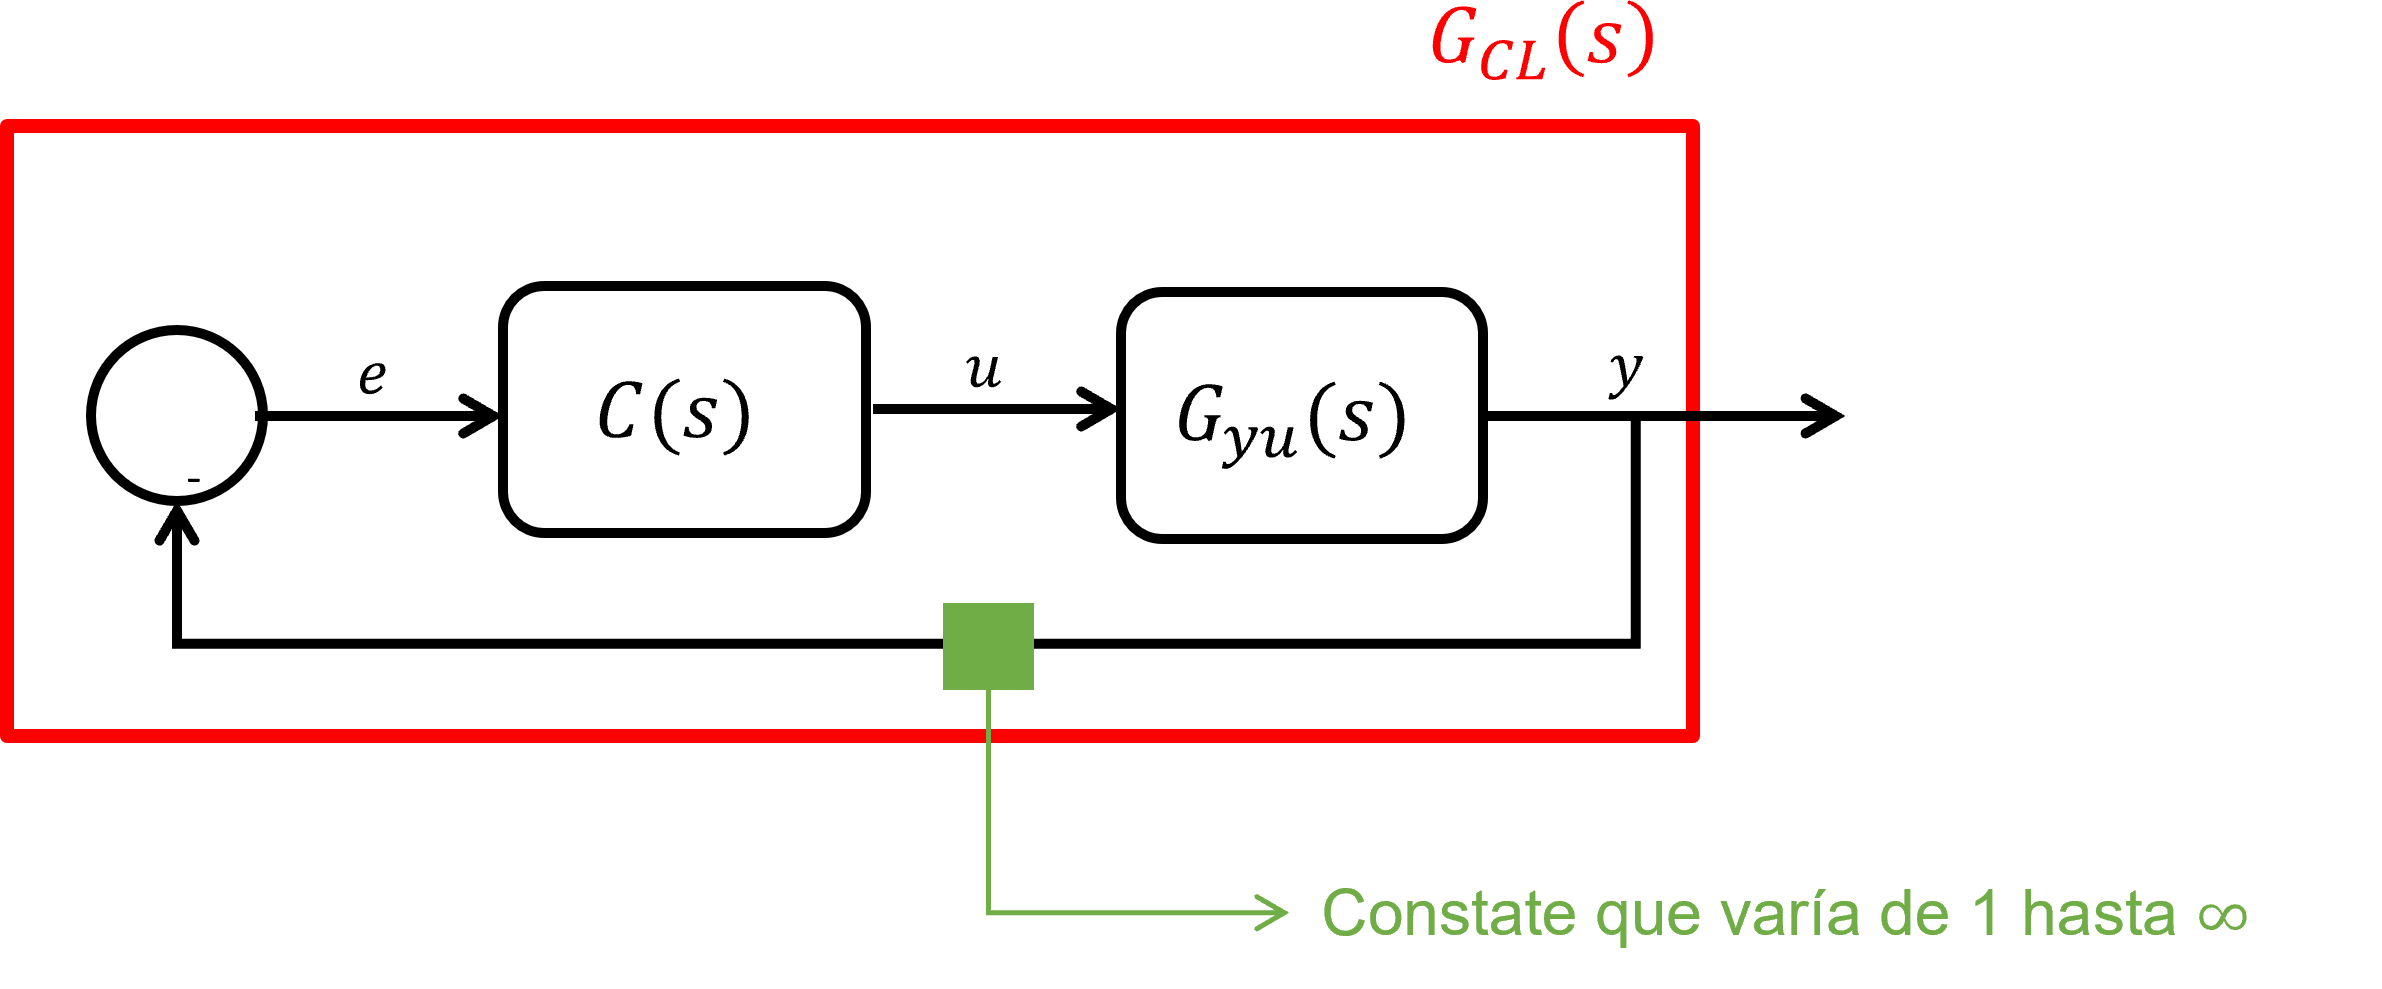
\includegraphics[scale=0.7]{Figuras/GCL.png}
\end{figure}

\begin{align*}
    G_{CL}(s)&=\frac{G(s)C(s)}{1+G(s)C(s)}\\
    G_{CL}(s)&=\frac{G(s)K_p\bigg(1+T_I/s+T_Ds\bigg)}{1+G(s)K_p\bigg(1+T_I/s+T_Ds\bigg)}
\end{align*}

\underline{Resumen control PID}: 
\begin{figure}[H]
\centering
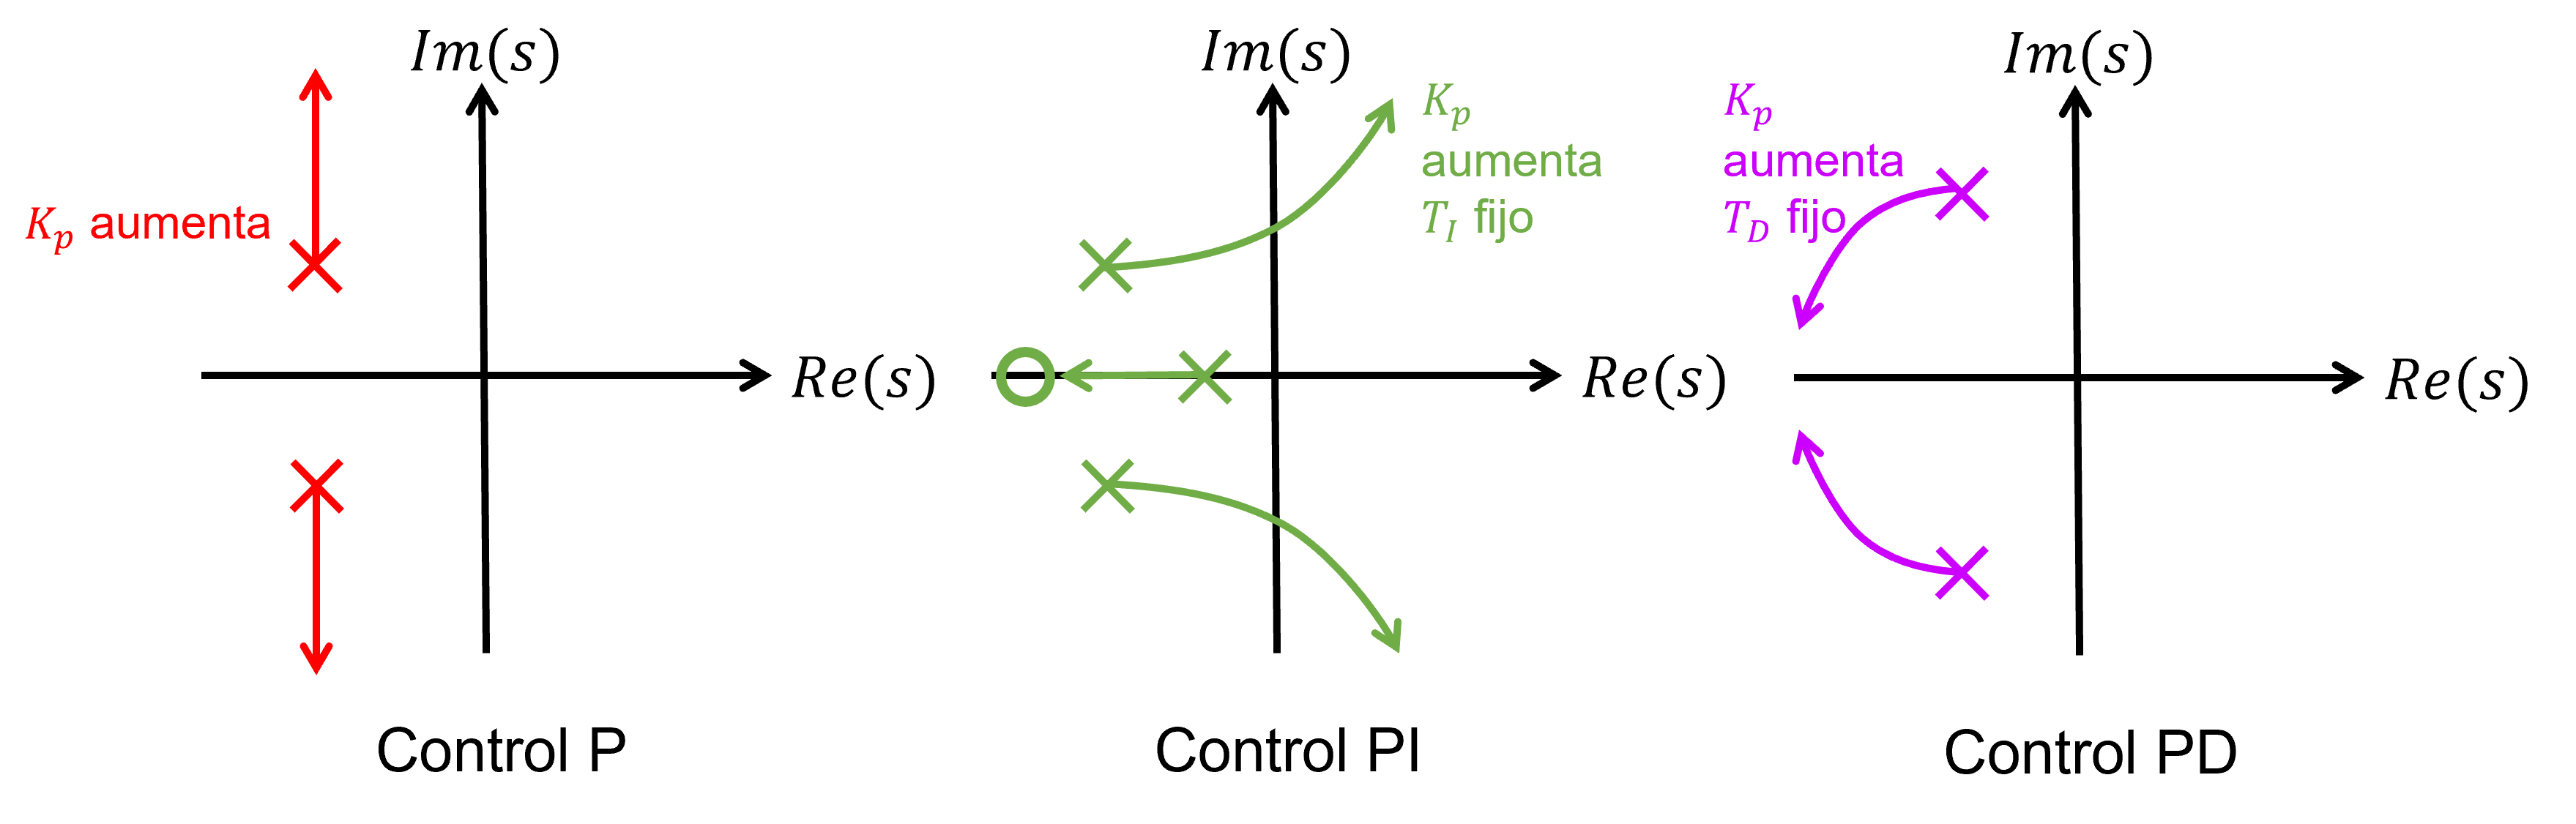
\includegraphics[scale=0.65]{Figuras/controlPID.png}
\end{figure}

\section{Control Moderno}
Representación espacio estado, sistema LTI.\\
\par Sea: 
\begin{align*}
    \tend{x}&=[x_1,x_2,...,x_N]^\top\\
    \tend{u}&=[u_1,u_2,...,u_p]^\top\\
    \tend{y}&=[y_1,y_2,...,y_r]^\top
\end{align*}
\begin{itemize}
    \item[(1)] Ecuación de estado:
    $$\tend{\dot{x}}=\tenq{A}\tend{x}+\tenq{B}\tend{u} $$
    \item[(2)] Ecuación de respuesta:
    $$\tend{y}=\tenq{C}\tend{x}+\tenq{D}\tend{u} $$
\end{itemize}

\underline{Paréntesis}:
\begin{align*}
    \tend{X}(s)&=\mathcal{L}\{\tend{x}(t)\}\\
    \tend{U}(s)&=\mathcal{L}\{\tend{u}(t)\}\\
    \tend{Y}(s)&=\mathcal{L}\{\tend{y}(t)\}
\end{align*}
\begin{align*}
    \tend{\dot{x}}\tenq{A}\tend{x}+\tenq{B}\tend{u}\xrightarrow[]{\mathcal{L}}s\tend{X}(s)=\tenq{A}\tend{X}(s)+\tenq{B}\tend{U}(s)\\
    \Longrightarrow \tend{X}(s)=(s\tenq{I}-\tenq{A})^{-1}\tenq{B}\tend{U}(s)\\
    G_{xu}(s)=(s\tenq{I}-\tenq{A})^{-1}\tenq{B}
\end{align*}
\begin{align*}
    \tend{y}=\tenq{C}\tend{x}+\tenq{D}\tend{u}\xrightarrow[]{\mathcal{L}}s\tend{Y}(s)=\tenq{C}\tend{X}(s)+\tenq{D}\tend{U}(s)\\
    \tenq{Y}(s)=[\tenq{C}(s\tenq{I}-\tenq{A})^{-1}\tenq{B}+\tenq{D}]\tend{U}(s)\\
    G_{yu}=\tenq{C}(s\tenq{I}-\tenq{A})^{-1}\tenq{B}+\tenq{D}
\end{align*}


\section{Formas canónicas}
\subsection{Forma Canónica Controlable (CCF)}
Asumir que $\tenq{D}=\tenq{0}$ (no hay componente ``feedthrough'' en la salida del sistema).
\begin{align*}
\tenq{A_c}=\left[
    \begin{array}{cccc|c}
     -a_1 & -a_2 & \dots & -a_{n-1} & -a_n\\ \hline
     1 & & & 0 & 0\\
       & 1 & & & \vdots\\
       & & \ddots & & \\
     0 & & & 1 & 0  
    \end{array}\right], \quad \tenq{A_c}\in \mathbb{R}^{n\times n}
\end{align*}
\begin{align*}
\tenq{B_c}=\left[
    \begin{array}{c}
     1 \\ \hline
     0\\
    \vdots\\
     0  
    \end{array}\right], \quad \tenq{B_c}\in \mathbb{R}^{n\times 1}
\end{align*}
\begin{align*}
\tenq{C_c}=\left[
    \begin{array}{cccc}
     b_1 & b_2 & \dots & b_n
    \end{array}\right], \quad \tenq{C_c}\in \mathbb{R}^{1\times n}
\end{align*}
\begin{align*}
    \text{Realización (SISO): }\quad 
    \left\{
    \begin{array}{l}
          \tend{\dot{x}_c}=\tenq{A_c}\tend{x_c}+\tenq{B_c}u \\
          y=\tenq{C_c}\tend{x_c} \\
    \end{array} 
    \right. 
\end{align*}
Notar que:
\begin{align*}
    \dot{x}_1 &= -a_1x_1-a_2x_2 ... -a_nx_n+1\cdot u\\
    \dot{x}_2 &= x_1\\
    \dot{x}_3 &= x_2\\
    \vdots \\
    \dot{x}_n &= x_{n-1}
\end{align*}

Utilizando la transformada de Laplace, se obtiene la siguiente función de transferencia:
\begin{align*}
    G_{yu}(s)=\frac{b_1s^{n-1}+b_2s^{n-2}+...+b-n}{s^n+a_1s^{n-1}+a_2s^{n-2}+...+a_n} = \frac{\text{numerador orden n-1}}{\text{denominador orden n}} = \text{TF Propia}
\end{align*}

Se utiliza para diseñar controladores cuando todos los estados del sistema son conocidos.

\subsection{Forma Canónica Modal (MCF)}
Sea $G(s)=\frac{c_1}{s+p_1}+\frac{c_2}{s+p_2}+...+\frac{c_n}{s+p_n}$, $G(s)$ se escribe como una expansión de fracción parcial, y los polos $p_i$ son todos distintos:
\begin{align*}
\tenq{A_m}=\left[
    \begin{array}{cccc}
     -p_1& & & 0\\
     & -p_2 & & \\
     & & \ddots & \\
     0 & & & -p_n
    \end{array}\right], \quad \tenq{A_m}\in \mathbb{R}^{n\times n}
\end{align*}
\begin{align*}
\tenq{B_m}=\left[
    \begin{array}{c}
     1 \\ 
     1\\
    \vdots\\
     1  
    \end{array}\right], \quad \tenq{B_m}\in \mathbb{R}^{n\times 1}
\end{align*}
\begin{align*}
\tenq{C_m}=\left[
    \begin{array}{cccc}
     c_1 & c_2 & \dots & c_n
    \end{array}\right], \quad \tenq{C_m}\in \mathbb{R}^{1\times n}
\end{align*}

\begin{align*}
    \text{Realización (SISO): }\quad 
    \left\{
    \begin{array}{l}
          \tend{\dot{x}_m}=\tenq{A_m}\tend{x_m}+\tenq{B_m}\cancelto{0}{u} 
    \end{array} 
    \right. 
\end{align*}

\begin{align*}
    \dot{x}_{m_1} &= \lambda_1x_{m_1}\\
    \dot{x}_{m_2} &= \lambda_2x_{m_1}\\
    \vdots \\
    \dot{x}_{m_n} &= \lambda_nx_{m_n}
\end{align*}

\begin{align*}
    \Longrightarrow\tend{\dot{x}}=\tenq{A}\tend{x}
\end{align*}

\underline{Resolver}: $\tenq{A}\tend{v}=\lambda \tend{v}$ (Problema de valores propios de $\tenq{A}$).\\
\par $\tenq{T}$ es la matriz de transformación modal, $\tenq{T}=[\tend{v_1},\tend{v_2},...,\tend{v_n}]$\\

\subsection{Forma Canónica Observable (OCF)}
Dado $G(s)=\frac{n(s)}{d(s)}$, con $a_i$, $b_i$ conocidos.

\begin{align*}
\tenq{A_o}=\left[
    \begin{array}{c|cccc}
     -a_{n-1} & 1 & & & 0 \\ 
     -a_{n-2} & & 1 & & \\
     \vdots   & & & \ddots & \\
     -a_1     & 0 & & & 1 \\ \hline
     -a_0     & 0 & 0 & \dots & 0   
    \end{array}\right], \quad \tenq{A_o}\in \mathbb{R}^{n\times n}
\end{align*}
\begin{align*}
\tenq{B_o}=\left[
    \begin{array}{c}
     b_{n-1} \\
     b_{n-2}\\
    \vdots\\
     b_1 \\ \hline
     b_0
    \end{array}\right], \quad \tenq{B_o}\in \mathbb{R}^{n\times 1}
\end{align*}
\begin{align*}
\tenq{C_o}=\left[
    \begin{array}{c|ccc}
     1 & 0 & \dots & 0
    \end{array}\right], \quad \tenq{C}_o\in \mathbb{R}^{1\times n}
\end{align*}

Se utiliza para diseñar ``observadores''.


\section{Control lazo cerrado utilizando estados (State Feedback Control)}

\begin{figure}[H]
\centering
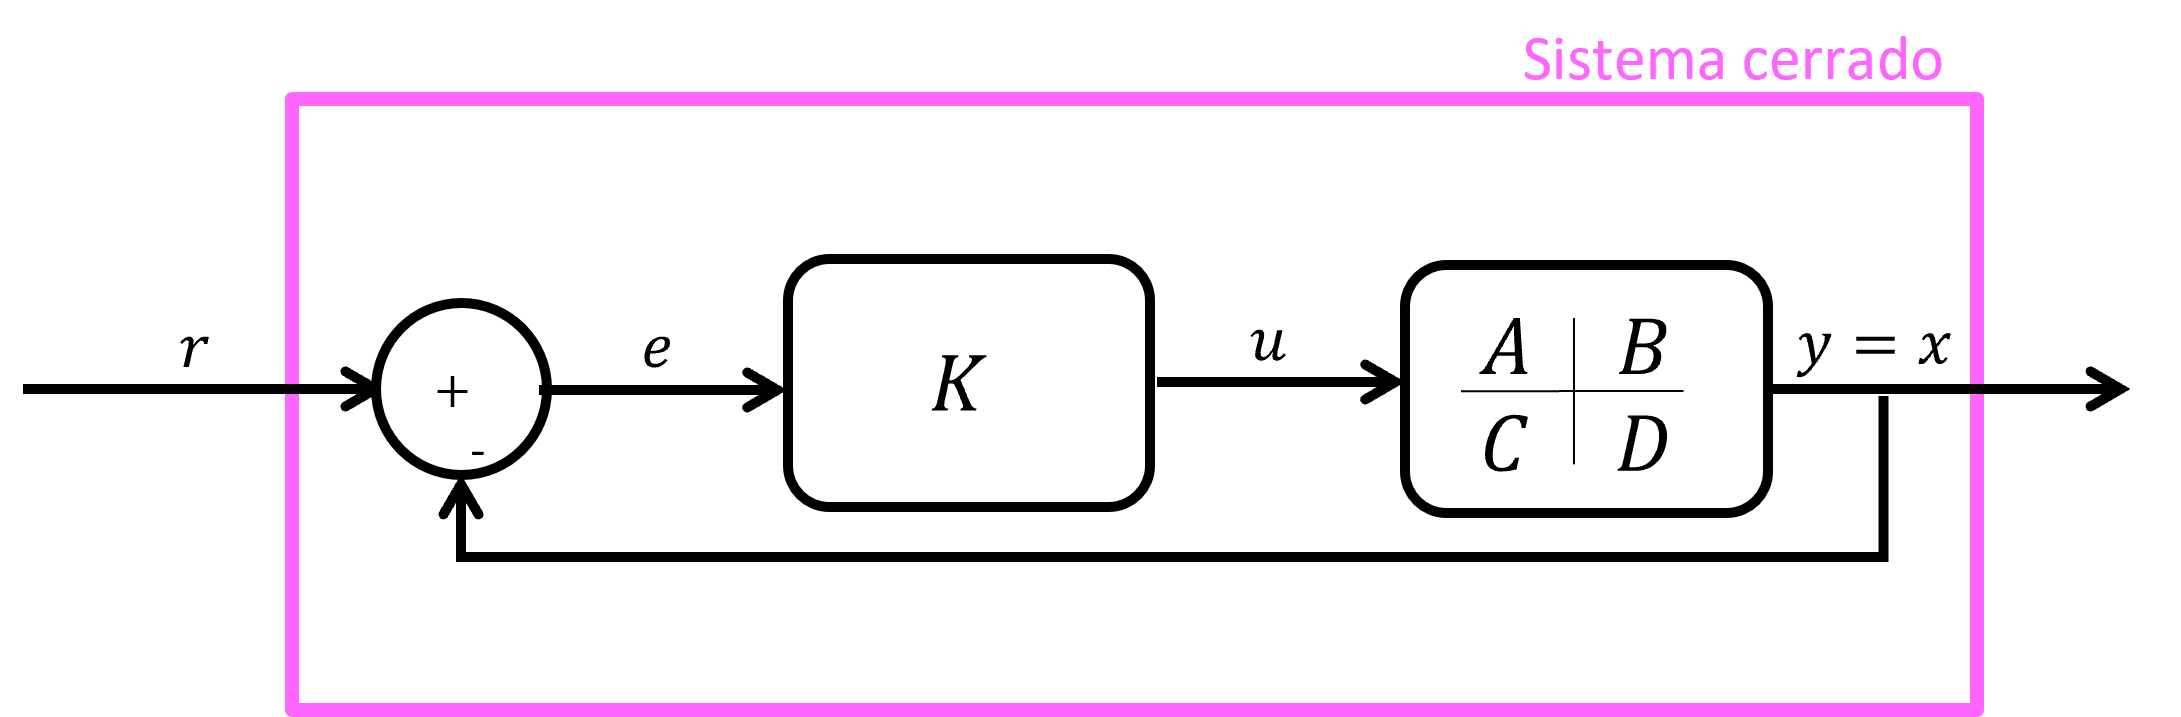
\includegraphics[scale=0.7]{Figuras/State_feedback.png}
\end{figure}
\underline{Objetivo}: Diseñar $K$ tal que $e=r-x\to 0$ para un tiempo $t_f$.\\
\par \underline{Definición}: El sistema de control ``full state feedback'' tiene relación con el hecho que el controlador cuenta con acceso a todos los estados del sistema.\\

\par Veamos la ecuación de estado del sistema:
\begin{align*}
    \dot{x}=Ax+Bu
\end{align*}
La señal de control:
\begin{align*}
    u=Ke
\end{align*}
La señal de error:
\begin{align*}
    e=r-x
\end{align*}

Luego:
\begin{align*}
    \dot{x} &= Ax+BK(r-x)\\
    \dot{x} &= (A-BK)x+BKr\\
\end{align*}
\begin{itemize}
    \item $A_{CL}=A-BK$: matriz de estado del sistema cerrado.
    \item $B_{CL}=BK$
\end{itemize}
\begin{align*}
    \dot{x}=A_{CL}x+B_{CL}r
\end{align*}
Para que el sistema cerrado sea \textcolor{red}{ESTABLE}, los valores propios de $A_{CL}$ deben tener partes reales estrictamente negativas:
\begin{align*}
    \text{Re}(eig(A_{CL}))<0
\end{align*}

\par Analicemos el diseño de un controlador utilizando una representación CCF:
\begin{align*}
\tenq{A}=\left[
    \begin{array}{cccc|c}
     -a_1 & -a_2 & \dots & -a_{n-1} & -a_n\\ \hline
     1 & & & 0 & 0\\
       & 1 & & & \vdots\\
       & & \ddots & & \\
     0 & & & 1 & 0  
    \end{array}\right]_{n\times n}
\end{align*}
\begin{align*}
\tenq{B}=\left[
    \begin{array}{c}
     1 \\ \hline
     0\\
    \vdots\\
     0  
    \end{array}\right]_{n\times 1}
\end{align*}
\begin{align*}
\tenq{K}=\left[
    \begin{array}{ccccc}
     k_{n-1} & k_{n-2} & \dots & k_1 & k_0
    \end{array}\right]_{1\times n}
\end{align*}

Calculemos $BK$:
\begin{align*}
\tenq{BK}=\left[
    \begin{array}{cccc|c}
     k_{n-1} & k_{n-2} & \dots & k_1 & k_0\\ \hline
      & & & & 0\\
      & & \tenq{0}_{(n-1)\times(n-1)} & & \vdots\\
      & & & & 0  
    \end{array}\right]_{n\times n}
\end{align*}

Ahora, calculemos $A_{CL}=A-BK$
\begin{align*}
\tenq{BK}=\left[
    \begin{array}{cccc|c}
     -(a_{n-1}+k_{n-1}) & -(a_{n-2}+k_{n-2}) & \dots & -(a_1+k_1) & -(a_0+k_0)\\ \hline
      & & & & 0\\
      & & \tenq{I}_{(n-1)\times(n-1)} & & \vdots\\
      & & & & 0  
    \end{array}\right]_{n\times n}
\end{align*}

Queremos encontrar los valores propios de $A_{CL}$. Escribamos la ecuación característica de $A_{CL}$
\begin{align*}
    \det(\tenq{A_{CL}}-\lambda \tenq{I})=0
\end{align*}

\begin{align*}
\tenq{BK}=\left[
    \begin{array}{cccc|c}
     -(\lambda+a_{n-1}+k_{n-1}) & -(a_{n-2}+k_{n-2}) & \dots & -(a_1+k_1) & -(a_0+k_0)\\ \hline
      1 & -\lambda & & & 0\\
      & 1 & -\lambda & & \vdots\\
      & & \ddots & \ddots & 0\\
      & & & 1 & -\lambda\\
    \end{array}\right]=0
\end{align*}

La ecuación característica resulta ser:
\begin{align*}
    \lambda^n+(a_{n-1}+k_{n-1})\lambda^{n-1}+(a_{n-2}+k_{n-2})\lambda^{n-2}+...+(a_{1}+k_{1})\lambda+(a_{0}+k_{0})=0
\end{align*}
Si queremos ubicar los polos en una posición particular, o sea, queremos fijar los polos de la siguiente manera:
$$ \lambda=\{p_1,p_2,p_3,..,p_n \}$$

Podemos reescribir la ecuación característica de la siguiente forma:
$$(\lambda-p_1)(\lambda-p_2)(\lambda-p_3)...(\lambda-p_n)=0 $$

Desarrollando el polinomio:
$$\Longrightarrow \lambda^n+\alpha_{n-1}\lambda^{n-1}+...+\alpha_1\lambda+\alpha_0=0 $$
Entonces, el controlador $K$ se define como:
\begin{align*}
    \alpha_{n-1} = a_{n-1}+k_{n-1} &\Longrightarrow k_{n-1} = \alpha_{n-1}-a_{n-1}\\
    \alpha_{n-2} = a_{n-2}+k_{n-2} &\Longrightarrow k_{n-2} = \alpha_{n-2}-a_{n-2}\\
    \vdots \\
    \alpha_0 = a_0+k_0 &\Longrightarrow k_0 = \alpha_0-a_0\\
\end{align*}
Donde $\alpha_i$ se obtiene de la posición deseada de los polos. \\
\par Entonces, si el sistema es CCF, podemos diseñar $K$ al elegir la posición de los polos de manera apropiada $\Longrightarrow$ \textcolor{red}{POLE PLACEMENT}\\
\par \underline{Nota}: Si el sistema no es CCF, entonces se puede transformar a CCF utilizando matriz de transformación $\tenq{T}$, provisto que el sistema sea controlable.\\
\par Sea la realización:
\begin{align*}
    \tend{x}=Ax+Bu \xrightarrow[]{x=Tz} \dot{z}=A_cz+B_cu
\end{align*}
Sea $T \in \mathbb{R}^{n\times n}$, tal que $T^{-1}$ existe
\begin{align*}
    \Longrightarrow x&=Tz\\
    \Longrightarrow \dot{x}&=T\dot{z}
\end{align*}
Reemplazando:
\begin{align*}
    T\dot{z} &= ATz+Bu\\
    \Longrightarrow \dot{z}&=T^{-1}ATz+T^{-1}Bu\\
    \dot{z} &= A_cz+B_cu
\end{align*}

``Pole placement'', pasos a seguir:
\begin{enumerate}
    \item Buscar $T$ y transformar a CCF ($A_c$ y $B_c$).
    \item Encontrar $K_c$ , en base a la ubicación de polos deseados.
    \item Volver al sistema original (asuma $r=0$)
\end{enumerate}
\begin{align*}
    \Longrightarrow \dot{z} &= (A_c-B_cK_c)z\\
    \Longrightarrow T\dot{z} &= TA_cz+TB_cz\\
    \Longrightarrow \dot{x} &= TT^{-1}ATz-TT^{-1}BK_cz\\
    \Longrightarrow \dot{x} &= Ax-BK_cT^{-1}x\\
    \Longrightarrow \dot{x} &= (A-BK)x
\end{align*}
donde  $K=K_cT^{-1}$, controlador para el sistema original.

